\begin{figure}[htbp]
  \centering
  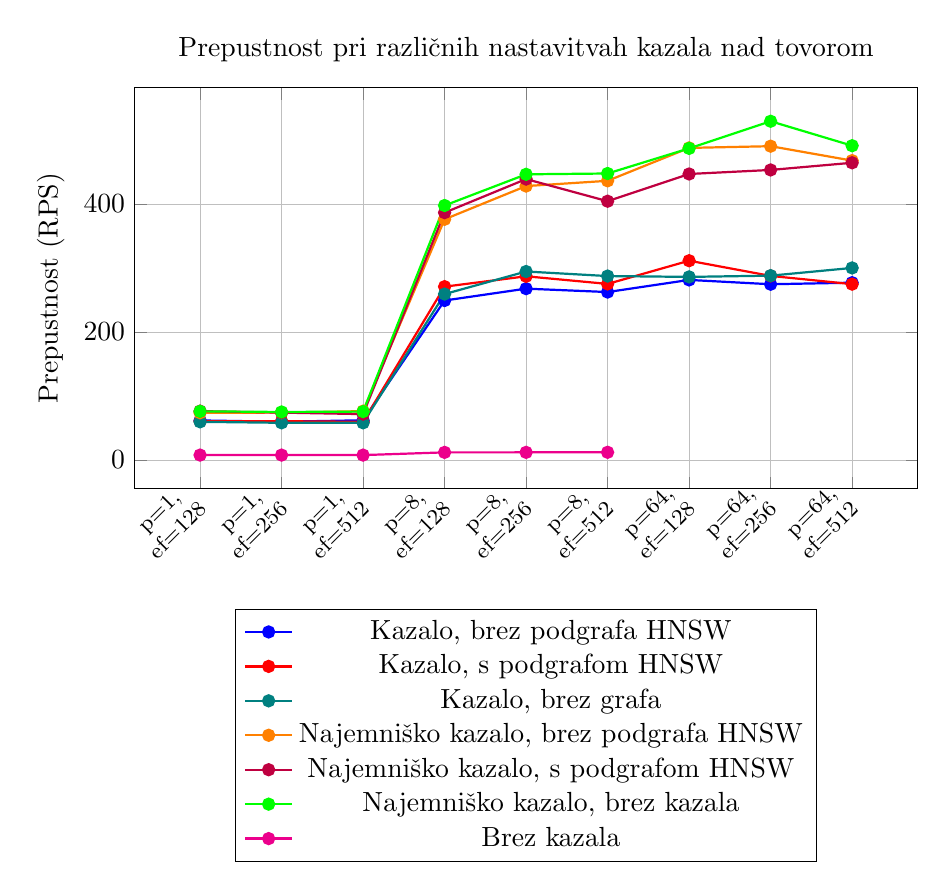
\begin{tikzpicture}
    \begin{axis}[
      title={Prepustnost pri različnih nastavitvah kazala nad tovorom},
      ylabel={Prepustnost (RPS)},
      symbolic x coords={
        p=1-ef128,
        p=1-ef256,
        p=1-ef512,
        p=8-ef128,
        p=8-ef256,
        p=8-ef512,
        p=64-ef128,
        p=64-ef256,
        p=64-ef512
      },
      xticklabels={
        {p=1,\\ef=128},
        {p=1,\\ef=256},
        {p=1,\\ef=512},
        {p=8,\\ef=128},
        {p=8,\\ef=256},
        {p=8,\\ef=512},
        {p=64,\\ef=128},
        {p=64,\\ef=256},
        {p=64,\\ef=512}
      },
      xtick=data,
      x tick label style={rotate=45, anchor=east, align=center, font=\footnotesize},
      /pgf/number format/use comma,
      /pgf/number format/fixed,
      /pgf/number format/precision=3,      grid=both,
      grid style={line width=.1pt, draw=gray!20},
      major grid style={line width=.2pt, draw=gray!50},
      legend style={at={(0.5, -0.30)}, anchor=north},
      width=0.95\textwidth,
      height=0.55\textwidth,
    ]

    % Series: Kazalo, brez podgrafa HNSW
    \addplot[color=blue, mark=*, thick] coordinates {
      (p=1-ef128, 61.5532)
      (p=1-ef256, 59.5190)
      (p=1-ef512, 61.7958)
      (p=8-ef128, 249.0277)
      (p=8-ef256, 267.5739)
      (p=8-ef512, 262.2629)
      (p=64-ef128, 281.2169)
      (p=64-ef256, 274.4674)
      (p=64-ef512, 276.8906)
    };
    \addlegendentry{Kazalo, brez podgrafa HNSW}

    % Series: Kazalo, s podgrafom HNSW
    \addplot[color=red, mark=*, thick] coordinates {
      (p=1-ef128, 60.4330)
      (p=1-ef256, 60.3655)
      (p=1-ef512, 59.3872)
      (p=8-ef128, 270.6852)
      (p=8-ef256, 286.8951)
      (p=8-ef512, 274.9632)
      (p=64-ef128, 311.2510)
      (p=64-ef256, 287.4843)
      (p=64-ef512, 274.6156)
    };
    \addlegendentry{Kazalo, s podgrafom HNSW}

    % Series: Kazalo, brez grafa
    \addplot[color=teal, mark=*, thick] coordinates {
      (p=1-ef128, 59.3706)
      (p=1-ef256, 57.8528)
      (p=1-ef512, 57.8306)
      (p=8-ef128, 259.1044)
      (p=8-ef256, 294.3694)
      (p=8-ef512, 287.2503)
      (p=64-ef128, 285.9632)
      (p=64-ef256, 287.8875)
      (p=64-ef512, 299.9662)
    };
    \addlegendentry{Kazalo, brez grafa}

    % Series: Najemniško kazalo, brez podgrafa HNSW
    \addplot[color=orange, mark=*, thick] coordinates {
      (p=1-ef128, 73.5607)
      (p=1-ef256, 73.7785)
      (p=1-ef512, 76.0855)
      (p=8-ef128, 376.0042)
      (p=8-ef256, 427.9403)
      (p=8-ef512, 436.1657)
      (p=64-ef128, 487.5981)
      (p=64-ef256, 490.2905)
      (p=64-ef512, 467.7273)
    };
    \addlegendentry{Najemniško kazalo, brez podgrafa HNSW}

    % Series: Najemniško kazalo, s podgrafom HNSW
    \addplot[color=purple, mark=*, thick] coordinates {
      (p=1-ef128, 76.1178)
      (p=1-ef256, 73.7784)
      (p=1-ef512, 71.4260)
      (p=8-ef128, 386.3971)
      (p=8-ef256, 438.8626)
      (p=8-ef512, 404.2585)
      (p=64-ef128, 446.8277)
      (p=64-ef256, 453.1399)
      (p=64-ef512, 464.3401)
    };
    \addlegendentry{Najemniško kazalo, s podgrafom HNSW}

    % Series: Najemniško kazalo, brez kazala
    \addplot[color=green, mark=*, thick] coordinates {
      (p=1-ef128, 75.8082)
      (p=1-ef256, 74.7845)
      (p=1-ef512, 75.3792)
      (p=8-ef128, 397.5443)
      (p=8-ef256, 446.3117)
      (p=8-ef512, 447.5962)
      (p=64-ef128, 486.8444)
      (p=64-ef256, 529.2581)
      (p=64-ef512, 491.0420)
    };
    \addlegendentry{Najemniško kazalo, brez kazala}

    % Series: Brez kazala
    \addplot[color=magenta, mark=*, thick] coordinates {
      (p=1-ef128, 7.4025)
      (p=1-ef256, 7.3828)
      (p=1-ef512, 7.3766)
      (p=8-ef128, 11.6099)
      (p=8-ef256, 11.6537)
      (p=8-ef512, 11.7609)
    };
    \addlegendentry{Brez kazala}
    \end{axis}
  \end{tikzpicture}
  \caption{Primerjava prepustnosti pri različnih nastavitvah kazala nad tovorom.}
  \label{fig:benchmark_kazalo_rps}
\end{figure}

\begin{figure}[htbp]
  \centering
  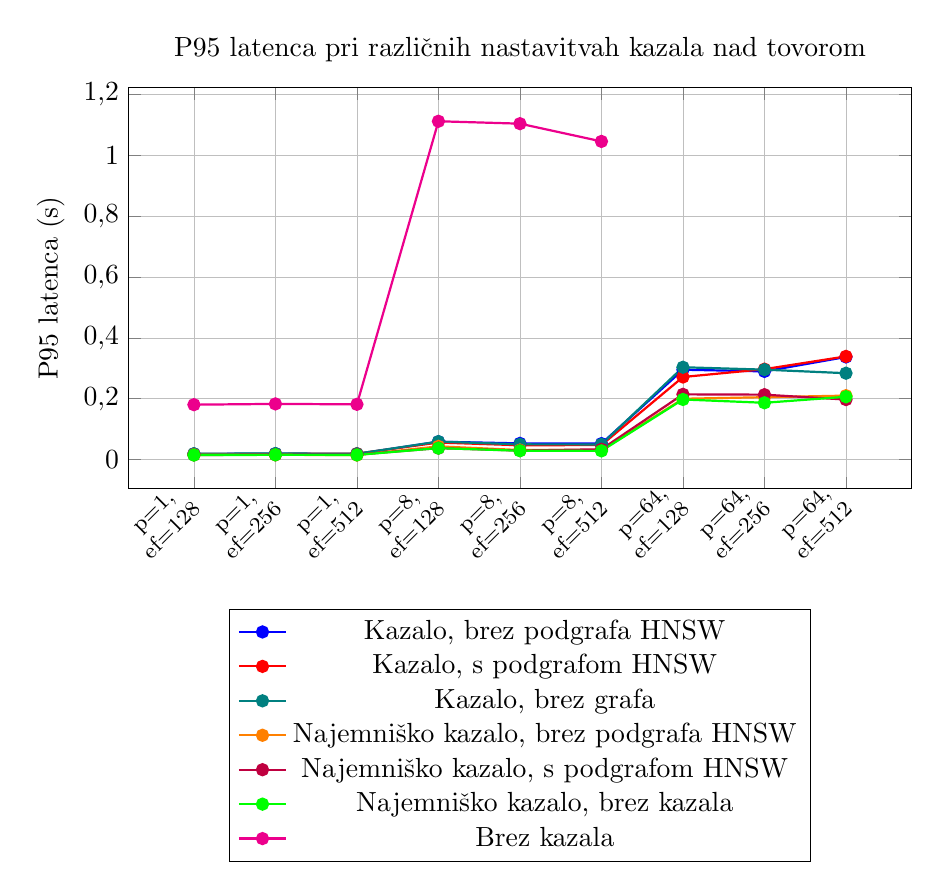
\begin{tikzpicture}
    \begin{axis}[
      title={P95 latenca pri različnih nastavitvah kazala nad tovorom},
      ylabel={P95 latenca (s)},
      symbolic x coords={
        p=1-ef128,
        p=1-ef256,
        p=1-ef512,
        p=8-ef128,
        p=8-ef256,
        p=8-ef512,
        p=64-ef128,
        p=64-ef256,
        p=64-ef512
      },
      xticklabels={
        {p=1,\\ef=128},
        {p=1,\\ef=256},
        {p=1,\\ef=512},
        {p=8,\\ef=128},
        {p=8,\\ef=256},
        {p=8,\\ef=512},
        {p=64,\\ef=128},
        {p=64,\\ef=256},
        {p=64,\\ef=512}
      },
      xtick=data,
      x tick label style={rotate=45, anchor=east, align=center, font=\footnotesize},
      /pgf/number format/use comma,
      /pgf/number format/fixed,
      /pgf/number format/precision=3,      grid=both,
      grid style={line width=.1pt, draw=gray!20},
      major grid style={line width=.2pt, draw=gray!50},
      legend style={at={(0.5, -0.30)}, anchor=north},
      width=0.95\textwidth,
      height=0.55\textwidth,
    ]

    % Series: Kazalo, brez podgrafa HNSW
    \addplot[color=blue, mark=*, thick] coordinates {
      (p=1-ef128, 0.0185)
      (p=1-ef256, 0.0193)
      (p=1-ef512, 0.0182)
      (p=8-ef128, 0.0588)
      (p=8-ef256, 0.0533)
      (p=8-ef512, 0.0525)
      (p=64-ef128, 0.2956)
      (p=64-ef256, 0.2901)
      (p=64-ef512, 0.3375)
    };
    \addlegendentry{Kazalo, brez podgrafa HNSW}

    % Series: Kazalo, s podgrafom HNSW
    \addplot[color=red, mark=*, thick] coordinates {
      (p=1-ef128, 0.0184)
      (p=1-ef256, 0.0187)
      (p=1-ef512, 0.0195)
      (p=8-ef128, 0.0561)
      (p=8-ef256, 0.0471)
      (p=8-ef512, 0.0478)
      (p=64-ef128, 0.2716)
      (p=64-ef256, 0.2974)
      (p=64-ef512, 0.3394)
    };
    \addlegendentry{Kazalo, s podgrafom HNSW}

    % Series: Kazalo, brez grafa
    \addplot[color=teal, mark=*, thick] coordinates {
      (p=1-ef128, 0.0193)
      (p=1-ef256, 0.0200)
      (p=1-ef512, 0.0191)
      (p=8-ef128, 0.0591)
      (p=8-ef256, 0.0501)
      (p=8-ef512, 0.0499)
      (p=64-ef128, 0.3037)
      (p=64-ef256, 0.2958)
      (p=64-ef512, 0.2841)
    };
    \addlegendentry{Kazalo, brez grafa}

    % Series: Najemniško kazalo, brez podgrafa HNSW
    \addplot[color=orange, mark=*, thick] coordinates {
      (p=1-ef128, 0.0161)
      (p=1-ef256, 0.0157)
      (p=1-ef512, 0.0149)
      (p=8-ef128, 0.0434)
      (p=8-ef256, 0.0314)
      (p=8-ef512, 0.0316)
      (p=64-ef128, 0.2000)
      (p=64-ef256, 0.2052)
      (p=64-ef512, 0.2103)
    };
    \addlegendentry{Najemniško kazalo, brez podgrafa HNSW}

    % Series: Najemniško kazalo, s podgrafom HNSW
    \addplot[color=purple, mark=*, thick] coordinates {
      (p=1-ef128, 0.0152)
      (p=1-ef256, 0.0158)
      (p=1-ef512, 0.0163)
      (p=8-ef128, 0.0376)
      (p=8-ef256, 0.0297)
      (p=8-ef512, 0.0339)
      (p=64-ef128, 0.2146)
      (p=64-ef256, 0.2135)
      (p=64-ef512, 0.1974)
    };
    \addlegendentry{Najemniško kazalo, s podgrafom HNSW}

    % Series: Najemniško kazalo, brez kazala
    \addplot[color=green, mark=*, thick] coordinates {
      (p=1-ef128, 0.0148)
      (p=1-ef256, 0.0156)
      (p=1-ef512, 0.0153)
      (p=8-ef128, 0.0377)
      (p=8-ef256, 0.0290)
      (p=8-ef512, 0.0286)
      (p=64-ef128, 0.1977)
      (p=64-ef256, 0.1868)
      (p=64-ef512, 0.2066)
    };
    \addlegendentry{Najemniško kazalo, brez kazala}

    % Series: Brez kazala
    \addplot[color=magenta, mark=*, thick] coordinates {
      (p=1-ef128, 0.1806)
      (p=1-ef256, 0.1831)
      (p=1-ef512, 0.1817)
      (p=8-ef128, 1.1128)
      (p=8-ef256, 1.1049)
      (p=8-ef512, 1.0465)
    };
    \addlegendentry{Brez kazala}
    \end{axis}
  \end{tikzpicture}
  \caption{Primerjava P95 latence pri različnih nastavitvah kazala nad tovorom.}
  \label{fig:benchmark_kazala_p95_time}
\end{figure}

\begin{figure}[htbp]
  \centering
  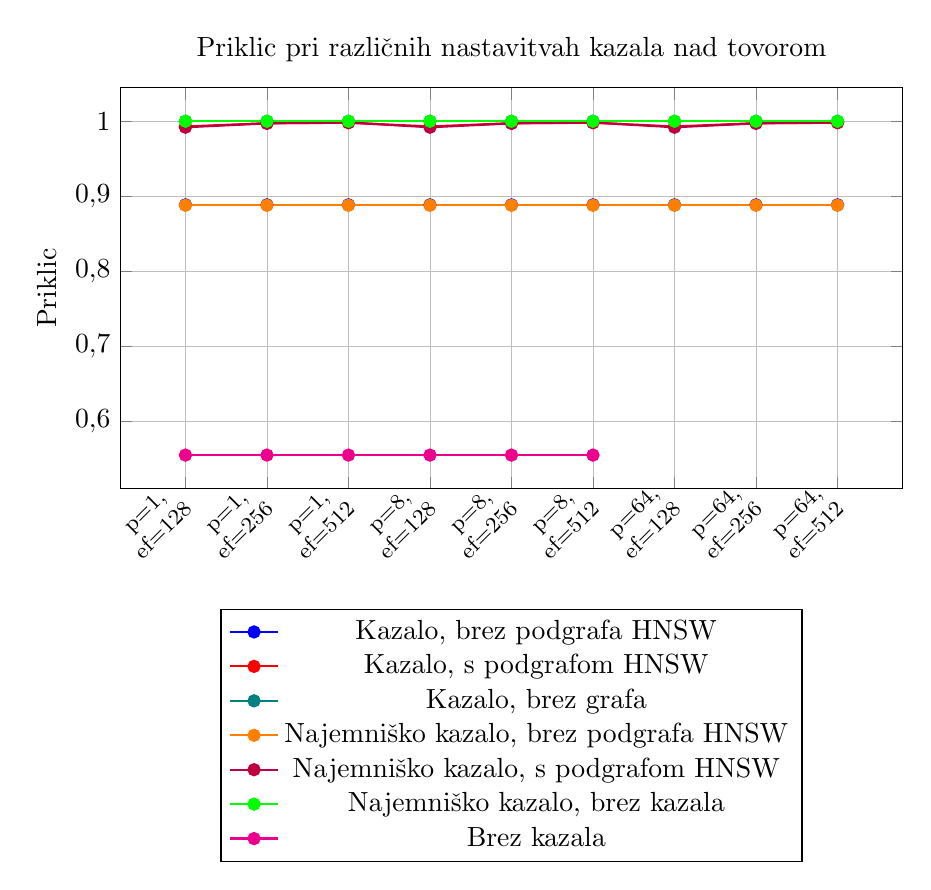
\begin{tikzpicture}
    \begin{axis}[
      title={Priklic pri različnih nastavitvah kazala nad tovorom},
      ylabel={Priklic},
      symbolic x coords={
        p=1-ef128,
        p=1-ef256,
        p=1-ef512,
        p=8-ef128,
        p=8-ef256,
        p=8-ef512,
        p=64-ef128,
        p=64-ef256,
        p=64-ef512
      },
      xticklabels={
        {p=1,\\ef=128},
        {p=1,\\ef=256},
        {p=1,\\ef=512},
        {p=8,\\ef=128},
        {p=8,\\ef=256},
        {p=8,\\ef=512},
        {p=64,\\ef=128},
        {p=64,\\ef=256},
        {p=64,\\ef=512}
      },
      xtick=data,
      x tick label style={rotate=45, anchor=east, align=center, font=\footnotesize},
      /pgf/number format/use comma,
      /pgf/number format/fixed,
      /pgf/number format/precision=3,      grid=both,
      grid style={line width=.1pt, draw=gray!20},
      major grid style={line width=.2pt, draw=gray!50},
      legend style={at={(0.5, -0.30)}, anchor=north},
      width=0.95\textwidth,
      height=0.55\textwidth,
    ]

    % Series: Kazalo, brez podgrafa HNSW
    \addplot[color=blue, mark=*, thick] coordinates {
      (p=1-ef128, 0.8884)
      (p=1-ef256, 0.8884)
      (p=1-ef512, 0.8884)
      (p=8-ef128, 0.8884)
      (p=8-ef256, 0.8884)
      (p=8-ef512, 0.8884)
      (p=64-ef128, 0.8884)
      (p=64-ef256, 0.8884)
      (p=64-ef512, 0.8884)
    };
    \addlegendentry{Kazalo, brez podgrafa HNSW}

    % Series: Kazalo, s podgrafom HNSW
    \addplot[color=red, mark=*, thick] coordinates {
      (p=1-ef128, 0.9930)
      (p=1-ef256, 0.9974)
      (p=1-ef512, 0.9980)
      (p=8-ef128, 0.9930)
      (p=8-ef256, 0.9974)
      (p=8-ef512, 0.9980)
      (p=64-ef128, 0.9930)
      (p=64-ef256, 0.9974)
      (p=64-ef512, 0.9980)
    };
    \addlegendentry{Kazalo, s podgrafom HNSW}

    % Series: Kazalo, brez grafa
    \addplot[color=teal, mark=*, thick] coordinates {
      (p=1-ef128, 1.0000)
      (p=1-ef256, 1.0000)
      (p=1-ef512, 1.0000)
      (p=8-ef128, 1.0000)
      (p=8-ef256, 1.0000)
      (p=8-ef512, 1.0000)
      (p=64-ef128, 1.0000)
      (p=64-ef256, 1.0000)
      (p=64-ef512, 1.0000)
    };
    \addlegendentry{Kazalo, brez grafa}

    % Series: Najemniško kazalo, brez podgrafa HNSW
    \addplot[color=orange, mark=*, thick] coordinates {
      (p=1-ef128, 0.8878)
      (p=1-ef256, 0.8878)
      (p=1-ef512, 0.8878)
      (p=8-ef128, 0.8878)
      (p=8-ef256, 0.8878)
      (p=8-ef512, 0.8878)
      (p=64-ef128, 0.8878)
      (p=64-ef256, 0.8878)
      (p=64-ef512, 0.8878)
    };
    \addlegendentry{Najemniško kazalo, brez podgrafa HNSW}

    % Series: Najemniško kazalo, s podgrafom HNSW
    \addplot[color=purple, mark=*, thick] coordinates {
      (p=1-ef128, 0.9920)
      (p=1-ef256, 0.9972)
      (p=1-ef512, 0.9984)
      (p=8-ef128, 0.9920)
      (p=8-ef256, 0.9972)
      (p=8-ef512, 0.9984)
      (p=64-ef128, 0.9920)
      (p=64-ef256, 0.9972)
      (p=64-ef512, 0.9984)
    };
    \addlegendentry{Najemniško kazalo, s podgrafom HNSW}

    % Series: Najemniško kazalo, brez kazala
    \addplot[color=green, mark=*, thick] coordinates {
      (p=1-ef128, 1.0000)
      (p=1-ef256, 1.0000)
      (p=1-ef512, 1.0000)
      (p=8-ef128, 1.0000)
      (p=8-ef256, 1.0000)
      (p=8-ef512, 1.0000)
      (p=64-ef128, 1.0000)
      (p=64-ef256, 1.0000)
      (p=64-ef512, 1.0000)
    };
    \addlegendentry{Najemniško kazalo, brez kazala}

    % Series: Brez kazala
    \addplot[color=magenta, mark=*, thick] coordinates {
      (p=1-ef128, 0.5542)
      (p=1-ef256, 0.5542)
      (p=1-ef512, 0.5542)
      (p=8-ef128, 0.5542)
      (p=8-ef256, 0.5542)
      (p=8-ef512, 0.5542)
    };
    \addlegendentry{Brez kazala}
    \end{axis}
  \end{tikzpicture}
  \caption{Primerjava priklica pri različnih nastavitvah kazala nad tovorom.}
  \label{fig:benchmark_todo_mean_precisions}
\end{figure}

\clearpage

\begin{figure}[htbp]
  \centering
  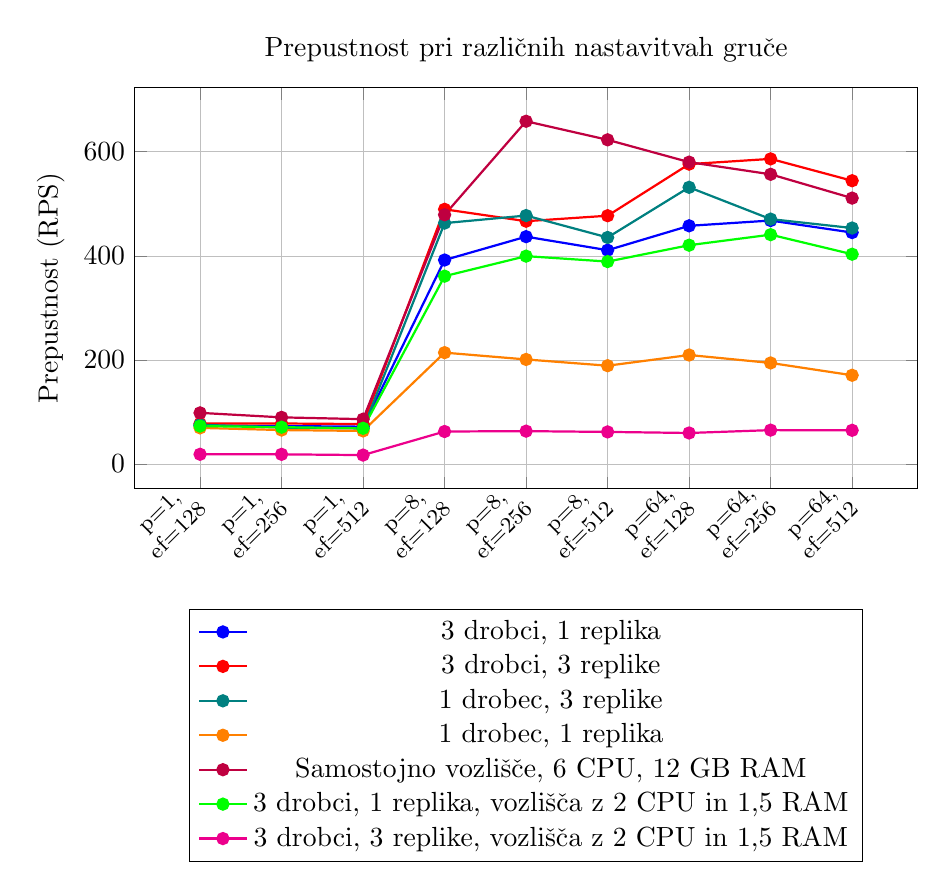
\begin{tikzpicture}
    \begin{axis}[
      title={Prepustnost pri različnih nastavitvah gruče},
      ylabel={Prepustnost (RPS)},
      symbolic x coords={
        p=1-ef128,
        p=1-ef256,
        p=1-ef512,
        p=8-ef128,
        p=8-ef256,
        p=8-ef512,
        p=64-ef128,
        p=64-ef256,
        p=64-ef512
      },
      xticklabels={
        {p=1,\\ef=128},
        {p=1,\\ef=256},
        {p=1,\\ef=512},
        {p=8,\\ef=128},
        {p=8,\\ef=256},
        {p=8,\\ef=512},
        {p=64,\\ef=128},
        {p=64,\\ef=256},
        {p=64,\\ef=512}
      },
      xtick=data,
      x tick label style={rotate=45, anchor=east, align=center, font=\footnotesize},
      /pgf/number format/use comma,
      /pgf/number format/fixed,
      /pgf/number format/precision=3,      grid=both,
      grid style={line width=.1pt, draw=gray!20},
      major grid style={line width=.2pt, draw=gray!50},
      legend style={at={(0.5, -0.30)}, anchor=north},
      width=0.95\textwidth,
      height=0.55\textwidth,
    ]

    % Series: cluster-2cpu-4ram/tenant/s3-r1/qdrant-dipl-sharding-3-shards-1-replica-tenant-m-16-ef-128-random-768-100-tenants-extended-upload-2026-08-17-15-58-42.json
    \addplot[color=blue, mark=*, thick] coordinates {
      (p=1-ef128, 73.9237)
      (p=1-ef256, 72.9634)
      (p=1-ef512, 71.8080)
      (p=8-ef128, 391.9236)
      (p=8-ef256, 436.7996)
      (p=8-ef512, 410.7921)
      (p=64-ef128, 457.6192)
      (p=64-ef256, 467.7762)
      (p=64-ef512, 444.6819)
    };
    \addlegendentry{3 drobci, 1 replika}

    % Series: cluster-2cpu-4ram/tenant/s3-r3/qdrant-dipl-sharding-3-shards-3-replica-tenant-m-16-ef-128-random-768-100-tenants-extended-upload-2026-08-19-11-03-15.json
    \addplot[color=red, mark=*, thick] coordinates {
      (p=1-ef128, 77.7705)
      (p=1-ef256, 77.8971)
      (p=1-ef512, 76.8138)
      (p=8-ef128, 489.3408)
      (p=8-ef256, 466.4942)
      (p=8-ef512, 477.0278)
      (p=64-ef128, 576.1238)
      (p=64-ef256, 586.1993)
      (p=64-ef512, 544.2456)
    };
    \addlegendentry{3 drobci, 3 replike}

    % Series: cluster-2cpu-4ram/tenant/s1-r3/qdrant-dipl-sharding-1-shard-3-replica-tenant-m-16-ef-128-random-768-100-tenants-extended-upload-2026-08-17-16-45-34.json
    \addplot[color=teal, mark=*, thick] coordinates {
      (p=1-ef128, 75.5708)
      (p=1-ef256, 69.9943)
      (p=1-ef512, 68.2909)
      (p=8-ef128, 462.8200)
      (p=8-ef256, 477.3430)
      (p=8-ef512, 435.2440)
      (p=64-ef128, 531.5843)
      (p=64-ef256, 470.4943)
      (p=64-ef512, 453.3652)
    };
    \addlegendentry{1 drobec, 3 replike}

    % Series: cluster-2cpu-4ram/tenant/s1-r1/qdrant-dipl-sharding-1-shard-1-replica-tenant-m-16-ef-128-random-768-100-tenants-extended-upload-2026-08-17-17-00-19.json
    \addplot[color=orange, mark=*, thick] coordinates {
      (p=1-ef128, 69.4912)
      (p=1-ef256, 65.2901)
      (p=1-ef512, 63.6394)
      (p=8-ef128, 214.0046)
      (p=8-ef256, 200.9295)
      (p=8-ef512, 188.9238)
      (p=64-ef128, 209.4525)
      (p=64-ef256, 194.2173)
      (p=64-ef512, 170.5526)
    };
    \addlegendentry{1 drobec, 1 replika}

    % Series: cluster-2cpu-4ram/tenant/single-node-6cpu-12-ram/qdrant-dipl-sharding-1-shard-1-replica-tenant-m-16-ef-128-random-768-100-tenants-extended-upload-2026-08-17-17-16-14.json
    \addplot[color=purple, mark=*, thick] coordinates {
      (p=1-ef128, 98.3283)
      (p=1-ef256, 89.6834)
      (p=1-ef512, 86.2206)
      (p=8-ef128, 478.8641)
      (p=8-ef256, 658.4759)
      (p=8-ef512, 622.8364)
      (p=64-ef128, 579.9571)
      (p=64-ef256, 556.5877)
      (p=64-ef512, 510.8574)
    };
    \addlegendentry{Samostojno vozlišče, 6 CPU, 12 GB RAM}

    % Series: cluster-2cpu-1.5ram/tenant-s3r1/qdrant-dipl-sharding-3-shards-1-replica-tenant-m-16-ef-128-random-768-100-tenants-extended-upload-2026-08-17-22-33-48.json
    \addplot[color=green, mark=*, thick] coordinates {
      (p=1-ef128, 72.9309)
      (p=1-ef256, 70.8272)
      (p=1-ef512, 68.7430)
      (p=8-ef128, 360.8961)
      (p=8-ef256, 399.3802)
      (p=8-ef512, 388.9212)
      (p=64-ef128, 420.3953)
      (p=64-ef256, 440.6081)
      (p=64-ef512, 403.0583)
    };
    \addlegendentry{3 drobci, 1 replika, vozlišča z 2 CPU in 1,5 RAM}

    % Series: cluster-2cpu-1.5ram/tenant-s3r3/qdrant-dipl-sharding-3-shards-3-replica-tenant-m-16-ef-128-random-768-100-tenants-extended-upload-2026-08-17-22-41-57.json
    \addplot[color=magenta, mark=*, thick] coordinates {
      (p=1-ef128, 18.7750)
      (p=1-ef256, 18.6672)
      (p=1-ef512, 17.2444)
      (p=8-ef128, 62.5155)
      (p=8-ef256, 63.2066)
      (p=8-ef512, 61.7312)
      (p=64-ef128, 59.6738)
      (p=64-ef256, 65.1710)
      (p=64-ef512, 64.8113)
    };
    \addlegendentry{3 drobci, 3 replike, vozlišča z 2 CPU in 1,5 RAM}
    \end{axis}
  \end{tikzpicture}
  \caption{Primerjava prepustnosti pri različnih nastavitvah gruče.}
  \label{fig:benchmark_todo_rps}
\end{figure}

\clearpage


\begin{figure}[htbp]
  \centering
  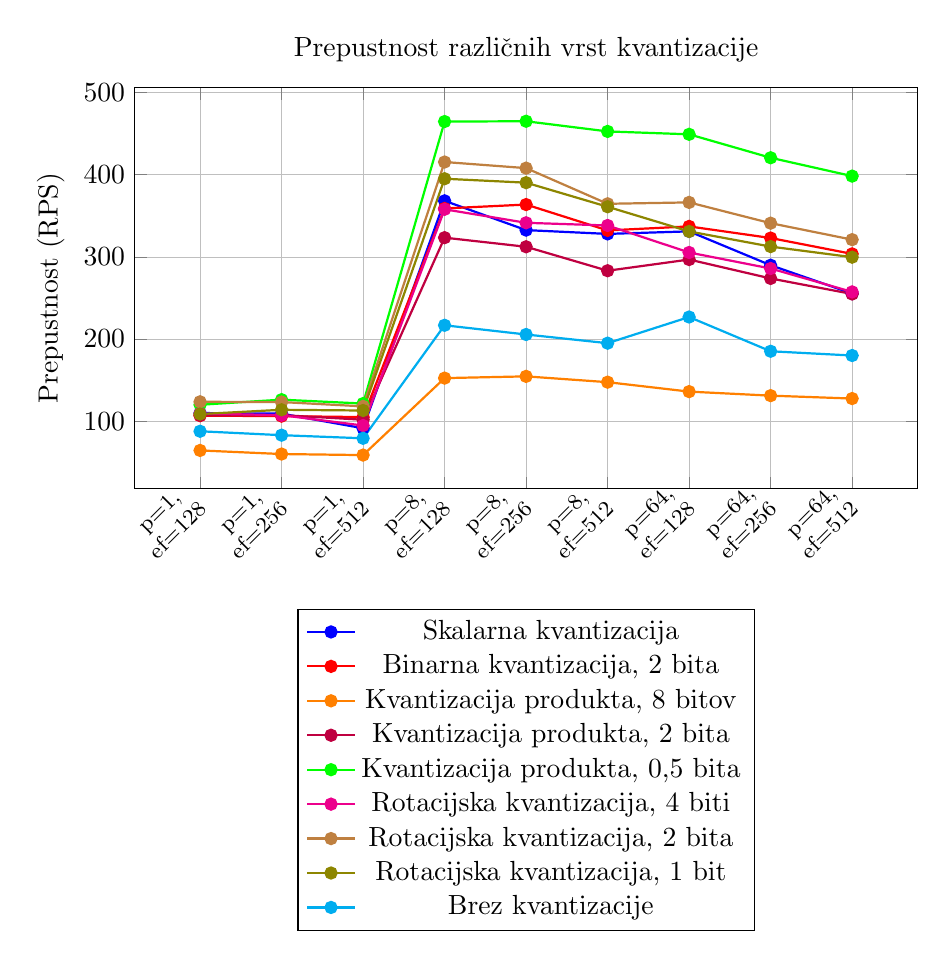
\begin{tikzpicture}
    \begin{axis}[
      title={Prepustnost različnih vrst kvantizacije},
      ylabel={Prepustnost (RPS)},
      symbolic x coords={
        p=1-ef128,
        p=1-ef256,
        p=1-ef512,
        p=8-ef128,
        p=8-ef256,
        p=8-ef512,
        p=64-ef128,
        p=64-ef256,
        p=64-ef512
      },
      xticklabels={
        {p=1,\\ef=128},
        {p=1,\\ef=256},
        {p=1,\\ef=512},
        {p=8,\\ef=128},
        {p=8,\\ef=256},
        {p=8,\\ef=512},
        {p=64,\\ef=128},
        {p=64,\\ef=256},
        {p=64,\\ef=512}
      },
      xtick=data,
      x tick label style={rotate=45, anchor=east, align=center, font=\footnotesize},
      /pgf/number format/use comma,
      /pgf/number format/fixed,
      /pgf/number format/precision=3,      grid=both,
      grid style={line width=.1pt, draw=gray!20},
      major grid style={line width=.2pt, draw=gray!50},
      legend style={at={(0.5, -0.30)}, anchor=north},
      width=0.95\textwidth,
      height=0.55\textwidth,
    ]

    % Series: Skalarna kvantizacija
    \addplot[color=blue, mark=*, thick] coordinates {
      (p=1-ef128, 109.9969)
      (p=1-ef256, 109.2352)
      (p=1-ef512, 91.4872)
      (p=8-ef128, 368.1626)
      (p=8-ef256, 332.5510)
      (p=8-ef512, 327.9221)
      (p=64-ef128, 331.0175)
      (p=64-ef256, 289.8241)
      (p=64-ef512, 255.3401)
    };
    \addlegendentry{Skalarna kvantizacija}

    % Series: Binarna kvantizacija, 2 bita
    \addplot[color=red, mark=*, thick] coordinates {
      (p=1-ef128, 106.8240)
      (p=1-ef256, 106.2346)
      (p=1-ef512, 105.0451)
      (p=8-ef128, 358.8963)
      (p=8-ef256, 363.6332)
      (p=8-ef512, 332.1681)
      (p=64-ef128, 337.0446)
      (p=64-ef256, 322.9195)
      (p=64-ef512, 303.6101)
    };
    \addlegendentry{Binarna kvantizacija, 2 bita}

    % Series: Kvantizacija produkta, 8 bitov
    \addplot[color=orange, mark=*, thick] coordinates {
      (p=1-ef128, 64.4942)
      (p=1-ef256, 60.1031)
      (p=1-ef512, 58.8443)
      (p=8-ef128, 152.4835)
      (p=8-ef256, 154.5980)
      (p=8-ef512, 147.5360)
      (p=64-ef128, 136.0608)
      (p=64-ef256, 131.1465)
      (p=64-ef512, 127.6170)
    };
    \addlegendentry{Kvantizacija produkta, 8 bitov}

    % Series: Kvantizacija produkta, 2 bita
    \addplot[color=purple, mark=*, thick] coordinates {
      (p=1-ef128, 107.2777)
      (p=1-ef256, 107.4588)
      (p=1-ef512, 101.8399)
      (p=8-ef128, 323.3456)
      (p=8-ef256, 312.2677)
      (p=8-ef512, 283.1158)
      (p=64-ef128, 296.7455)
      (p=64-ef256, 273.7228)
      (p=64-ef512, 254.8108)
    };
    \addlegendentry{Kvantizacija produkta, 2 bita}

    % Series: Kvantizacija produkta, 0,5 bita
    \addplot[color=green, mark=*, thick] coordinates {
      (p=1-ef128, 120.0482)
      (p=1-ef256, 126.2701)
      (p=1-ef512, 121.5201)
      (p=8-ef128, 464.6204)
      (p=8-ef256, 464.9708)
      (p=8-ef512, 452.6066)
      (p=64-ef128, 449.0773)
      (p=64-ef256, 420.5658)
      (p=64-ef512, 398.2455)
    };
    \addlegendentry{Kvantizacija produkta, 0,5 bita}

    % Series: Rotacijska kvantizacija, 4 biti
    \addplot[color=magenta, mark=*, thick] coordinates {
      (p=1-ef128, 109.4242)
      (p=1-ef256, 107.3792)
      (p=1-ef512, 94.7944)
      (p=8-ef128, 357.8579)
      (p=8-ef256, 341.4316)
      (p=8-ef512, 338.1671)
      (p=64-ef128, 305.3127)
      (p=64-ef256, 285.8259)
      (p=64-ef512, 257.3734)
    };
    \addlegendentry{Rotacijska kvantizacija, 4 biti}

    % Series: Rotacijska kvantizacija, 2 bita
    \addplot[color=brown, mark=*, thick] coordinates {
      (p=1-ef128, 123.6831)
      (p=1-ef256, 123.3374)
      (p=1-ef512, 118.1266)
      (p=8-ef128, 415.3819)
      (p=8-ef256, 407.9535)
      (p=8-ef512, 364.5487)
      (p=64-ef128, 366.2496)
      (p=64-ef256, 340.9769)
      (p=64-ef512, 320.9392)
    };
    \addlegendentry{Rotacijska kvantizacija, 2 bita}

    % Series: Rotacijska kvantizacija, 1 bit
    \addplot[color=olive, mark=*, thick] coordinates {
      (p=1-ef128, 108.7442)
      (p=1-ef256, 113.9424)
      (p=1-ef512, 113.0558)
      (p=8-ef128, 395.0465)
      (p=8-ef256, 390.2434)
      (p=8-ef512, 360.9439)
      (p=64-ef128, 330.9212)
      (p=64-ef256, 312.4820)
      (p=64-ef512, 299.6072)
    };
    \addlegendentry{Rotacijska kvantizacija, 1 bit}

    % Series: Brez kvantizacije
    \addplot[color=cyan, mark=*, thick] coordinates {
      (p=1-ef128, 87.8155)
      (p=1-ef256, 83.0471)
      (p=1-ef512, 79.2735)
      (p=8-ef128, 216.7498)
      (p=8-ef256, 205.5438)
      (p=8-ef512, 194.9752)
      (p=64-ef128, 226.8105)
      (p=64-ef256, 185.1397)
      (p=64-ef512, 179.9684)
    };
    \addlegendentry{Brez kvantizacije}
    \end{axis}
  \end{tikzpicture}
  \caption{Primerjava prepustnosti pri različnih vrstah kvantizacije, samostojno vozlišče 2 CPU in 4 GB RAM. Faktor vzorčenja $v = 2,0$.}
  \label{fig:benchmark_todo_rps}
\end{figure}

\begin{figure}[htbp]
  \centering
  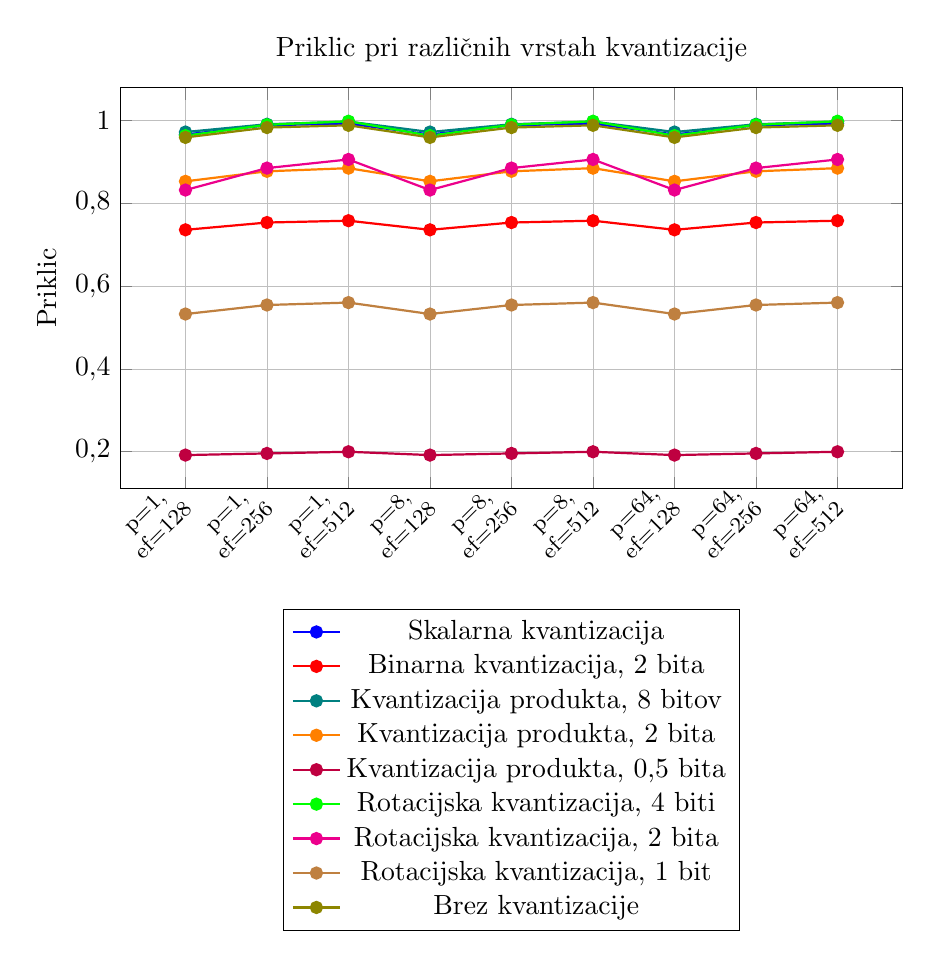
\begin{tikzpicture}
    \begin{axis}[
      title={Priklic pri različnih vrstah kvantizacije},
      ylabel={Priklic},
      symbolic x coords={
        p=1-ef128,
        p=1-ef256,
        p=1-ef512,
        p=8-ef128,
        p=8-ef256,
        p=8-ef512,
        p=64-ef128,
        p=64-ef256,
        p=64-ef512
      },
      xticklabels={
        {p=1,\\ef=128},
        {p=1,\\ef=256},
        {p=1,\\ef=512},
        {p=8,\\ef=128},
        {p=8,\\ef=256},
        {p=8,\\ef=512},
        {p=64,\\ef=128},
        {p=64,\\ef=256},
        {p=64,\\ef=512}
      },
      xtick=data,
      x tick label style={rotate=45, anchor=east, align=center, font=\footnotesize},
      /pgf/number format/use comma,
      /pgf/number format/fixed,
      /pgf/number format/precision=3,      grid=both,
      grid style={line width=.1pt, draw=gray!20},
      major grid style={line width=.2pt, draw=gray!50},
      legend style={at={(0.5, -0.30)}, anchor=north},
      width=0.95\textwidth,
      height=0.55\textwidth,
    ]

    % Series: Skalarna kvantizacija
    \addplot[color=blue, mark=*, thick] coordinates {
      (p=1-ef128, 0.9654)
      (p=1-ef256, 0.9878)
      (p=1-ef512, 0.9918)
      (p=8-ef128, 0.9654)
      (p=8-ef256, 0.9878)
      (p=8-ef512, 0.9918)
      (p=64-ef128, 0.9654)
      (p=64-ef256, 0.9878)
      (p=64-ef512, 0.9918)
    };
    \addlegendentry{Skalarna kvantizacija}

    % Series: Binarna kvantizacija, 2 bita
    \addplot[color=red, mark=*, thick] coordinates {
      (p=1-ef128, 0.7354)
      (p=1-ef256, 0.7530)
      (p=1-ef512, 0.7574)
      (p=8-ef128, 0.7354)
      (p=8-ef256, 0.7530)
      (p=8-ef512, 0.7574)
      (p=64-ef128, 0.7354)
      (p=64-ef256, 0.7530)
      (p=64-ef512, 0.7574)
    };
    \addlegendentry{Binarna kvantizacija, 2 bita}

    % Series: Kvantizacija produkta, 8 bitov
    \addplot[color=teal, mark=*, thick] coordinates {
      (p=1-ef128, 0.9714)
      (p=1-ef256, 0.9902)
      (p=1-ef512, 0.9966)
      (p=8-ef128, 0.9714)
      (p=8-ef256, 0.9902)
      (p=8-ef512, 0.9966)
      (p=64-ef128, 0.9714)
      (p=64-ef256, 0.9902)
      (p=64-ef512, 0.9966)
    };
    \addlegendentry{Kvantizacija produkta, 8 bitov}

    % Series: Kvantizacija produkta, 2 bita
    \addplot[color=orange, mark=*, thick] coordinates {
      (p=1-ef128, 0.8524)
      (p=1-ef256, 0.8766)
      (p=1-ef512, 0.8842)
      (p=8-ef128, 0.8524)
      (p=8-ef256, 0.8766)
      (p=8-ef512, 0.8842)
      (p=64-ef128, 0.8524)
      (p=64-ef256, 0.8766)
      (p=64-ef512, 0.8842)
    };
    \addlegendentry{Kvantizacija produkta, 2 bita}

    % Series: Kvantizacija produkta, 0,5 bita
    \addplot[color=purple, mark=*, thick] coordinates {
      (p=1-ef128, 0.1918)
      (p=1-ef256, 0.1958)
      (p=1-ef512, 0.1998)
      (p=8-ef128, 0.1918)
      (p=8-ef256, 0.1958)
      (p=8-ef512, 0.1998)
      (p=64-ef128, 0.1918)
      (p=64-ef256, 0.1958)
      (p=64-ef512, 0.1998)
    };
    \addlegendentry{Kvantizacija produkta, 0,5 bita}

    % Series: Rotacijska kvantizacija, 4 biti
    \addplot[color=green, mark=*, thick] coordinates {
      (p=1-ef128, 0.9626)
      (p=1-ef256, 0.9888)
      (p=1-ef512, 0.9974)
      (p=8-ef128, 0.9626)
      (p=8-ef256, 0.9888)
      (p=8-ef512, 0.9974)
      (p=64-ef128, 0.9626)
      (p=64-ef256, 0.9888)
      (p=64-ef512, 0.9974)
    };
    \addlegendentry{Rotacijska kvantizacija, 4 biti}

    % Series: Rotacijska kvantizacija, 2 bita
    \addplot[color=magenta, mark=*, thick] coordinates {
      (p=1-ef128, 0.8314)
      (p=1-ef256, 0.8844)
      (p=1-ef512, 0.9052)
      (p=8-ef128, 0.8314)
      (p=8-ef256, 0.8844)
      (p=8-ef512, 0.9052)
      (p=64-ef128, 0.8314)
      (p=64-ef256, 0.8844)
      (p=64-ef512, 0.9052)
    };
    \addlegendentry{Rotacijska kvantizacija, 2 bita}

    % Series: Rotacijska kvantizacija, 1 bit
    \addplot[color=brown, mark=*, thick] coordinates {
      (p=1-ef128, 0.5322)
      (p=1-ef256, 0.5540)
      (p=1-ef512, 0.5598)
      (p=8-ef128, 0.5322)
      (p=8-ef256, 0.5540)
      (p=8-ef512, 0.5598)
      (p=64-ef128, 0.5322)
      (p=64-ef256, 0.5540)
      (p=64-ef512, 0.5598)
    };
    \addlegendentry{Rotacijska kvantizacija, 1 bit}

    % Series: Brez kvantizacije
    \addplot[color=olive, mark=*, thick] coordinates {
      (p=1-ef128, 0.9584)
      (p=1-ef256, 0.9822)
      (p=1-ef512, 0.9876)
      (p=8-ef128, 0.9584)
      (p=8-ef256, 0.9822)
      (p=8-ef512, 0.9876)
      (p=64-ef128, 0.9584)
      (p=64-ef256, 0.9822)
      (p=64-ef512, 0.9876)
    };
    \addlegendentry{Brez kvantizacije}
    \end{axis}
  \end{tikzpicture}
  \caption{Priklic pri različnih vrstah kvantizacije, samostojno vozlišče 2 CPU in 4 GB RAM. Faktor vzorčenja $v = 0,2$.}
  \label{fig:benchmark_todo_mean_precisions}
\end{figure}

\begin{figure}[htbp]
  \centering
  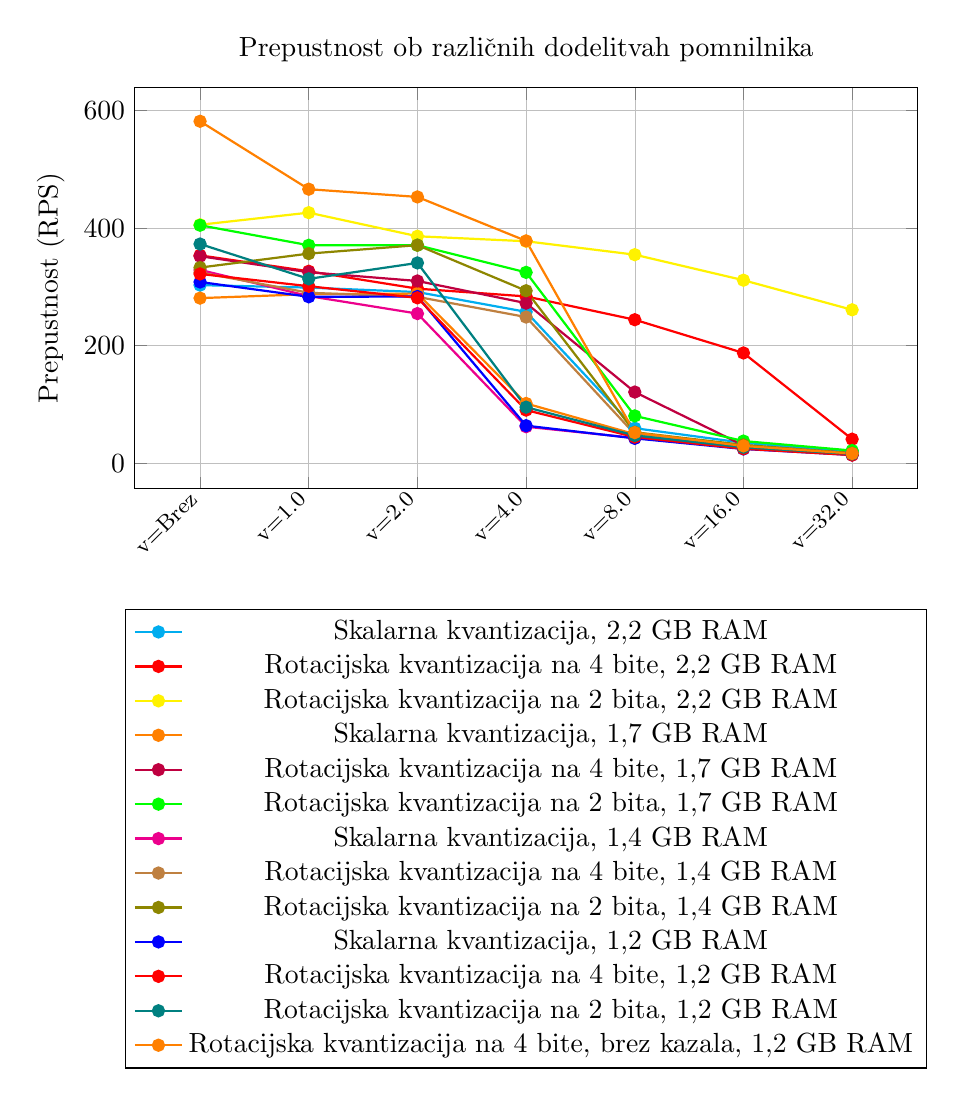
\begin{tikzpicture}
    \begin{axis}[
      title={Prepustnost ob različnih dodelitvah pomnilnika},
      ylabel={Prepustnost (RPS)},
      symbolic x coords={
        vnull,
        v1.0,
        v2.0,
        v4.0,
        v8.0,
        v16.0,
        v32.0,
      },
      xticklabels={
        {v=Brez},
        {v=1.0},
        {v=2.0},
        {v=4.0},
        {v=8.0},
        {v=16.0},
        {v=32.0}
      },
      xtick=data,
      x tick label style={rotate=45, anchor=east, align=center, font=\footnotesize},
      /pgf/number format/use comma,
      /pgf/number format/fixed,
      /pgf/number format/precision=3,      grid=both,
      grid style={line width=.1pt, draw=gray!20},
      major grid style={line width=.2pt, draw=gray!50},
      legend style={at={(0.5, -0.30)}, anchor=north},
      width=0.95\textwidth,
      height=0.55\textwidth,
    ]

    % Series: Skalarna kvantizacija, 2, GB RAM
    \addplot[color=cyan, mark=*, thick] coordinates {
      (vnull, 303.1286)
      (v1.0, 298.9116)
      (v2.0, 291.3495)
      (v4.0, 257.6954)
      (v8.0, 59.8532)
      (v16.0, 35.0105)
      (v32.0, 20.6449)
    };
    \addlegendentry{Skalarna kvantizacija, 2,2 GB RAM}

    % Series: Rotacijska kvantizacija na 4 bite, 2,2 GB RAM
    \addplot[color=red, mark=*, thick] coordinates {
      (vnull, 353.7137)
      (v1.0, 326.6954)
      (v2.0, 297.1088)
      (v4.0, 283.9080)
      (v8.0, 244.2856)
      (v16.0, 187.7566)
      (v32.0, 41.1977)
    };
    \addlegendentry{Rotacijska kvantizacija na 4 bite, 2,2 GB RAM}

    % Series: Rotacijska kvantizacija na 2 bita, 2,2 GB RAM
    \addplot[color=yellow, mark=*, thick] coordinates {
      (vnull, 405.7338)
      (v1.0, 426.3216)
      (v2.0, 386.1879)
      (v4.0, 377.7223)
      (v8.0, 354.8914)
      (v16.0, 311.4694)
      (v32.0, 261.1585)
    };
    \addlegendentry{Rotacijska kvantizacija na 2 bita, 2,2 GB RAM}

    % Series: Skalarna kvantizacija, 1,7 GB RAM
    \addplot[color=orange, mark=*, thick] coordinates {
      (vnull, 281.0156)
      (v1.0, 287.7506)
      (v2.0, 288.7166)
      (v4.0, 101.9174)
      (v8.0, 49.6295)
      (v16.0, 29.3668)
      (v32.0, 16.9126)
    };
    \addlegendentry{Skalarna kvantizacija, 1,7 GB RAM}

    % Series: Rotacijska kvantizacija na 4 bite, 1,7 GB RAM
    \addplot[color=purple, mark=*, thick] coordinates {
      (vnull, 352.2756)
      (v1.0, 325.0040)
      (v2.0, 310.1677)
      (v4.0, 272.4349)
      (v8.0, 121.3210)
      (v16.0, 30.5835)
      (v32.0, 17.3329)
    };
    \addlegendentry{Rotacijska kvantizacija na 4 bite, 1,7 GB RAM}

    % Series: Rotacijska kvantizacija na 2 bita, 1,7 GB RAM
    \addplot[color=green, mark=*, thick] coordinates {
      (vnull, 404.9143)
      (v1.0, 370.8909)
      (v2.0, 370.9902)
      (v4.0, 324.7901)
      (v8.0, 80.7713)
      (v16.0, 37.9946)
      (v32.0, 21.8426)
    };
    \addlegendentry{Rotacijska kvantizacija na 2 bita, 1,7 GB RAM}

    % Series: Skalarna kvantizacija, 1,4 GB RAM
    \addplot[color=magenta, mark=*, thick] coordinates {
      (vnull, 328.9937)
      (v1.0, 284.4947)
      (v2.0, 254.7136)
      (v4.0, 62.3949)
      (v8.0, 43.2334)
      (v16.0, 25.8227)
      (v32.0, 15.0849)
    };
    \addlegendentry{Skalarna kvantizacija, 1,4 GB RAM}

    % Series: Rotacijska kvantizacija na 4 bite, 1,4 GB RAM
    \addplot[color=brown, mark=*, thick] coordinates {
      (vnull, 324.6550)
      (v1.0, 290.1410)
      (v2.0, 283.1567)
      (v4.0, 248.8283)
      (v8.0, 49.7628)
      (v16.0, 27.2354)
      (v32.0, 16.5459)
    };
    \addlegendentry{Rotacijska kvantizacija na 4 bite, 1,4 GB RAM}

    % Series: Rotacijska kvantizacija na 2 bita, 1,4 GB RAM
    \addplot[color=olive, mark=*, thick] coordinates {
      (vnull, 332.9773)
      (v1.0, 356.7020)
      (v2.0, 371.0703)
      (v4.0, 293.5404)
      (v8.0, 52.9437)
      (v16.0, 31.4480)
      (v32.0, 17.4162)
    };
    \addlegendentry{Rotacijska kvantizacija na 2 bita, 1,4 GB RAM}

    % Series: Skalarna kvantizacija, 1,2 GB RAM
    \addplot[color=blue, mark=*, thick] coordinates {
      (vnull, 308.4515)
      (v1.0, 283.2663)
      (v2.0, 283.7407)
      (v4.0, 64.1327)
      (v8.0, 42.5738)
      (v16.0, 24.5048)
      (v32.0, 14.3456)
    };
    \addlegendentry{Skalarna kvantizacija, 1,2 GB RAM}

    % Series: Rotacijska kvantizacija na 4 bite, 1,2 GB RAM
    \addplot[color=red, mark=*, thick] coordinates {
      (vnull, 322.1524)
      (v1.0, 301.2405)
      (v2.0, 281.5185)
      (v4.0, 90.6148)
      (v8.0, 44.7847)
      (v16.0, 24.9387)
      (v32.0, 14.1302)
    };
    \addlegendentry{Rotacijska kvantizacija na 4 bite, 1,2 GB RAM}

    % Series: Rotacijska kvantizacija na 2 bita, 1,2 GB RAM
    \addplot[color=teal, mark=*, thick] coordinates {
      (vnull, 372.9866)
      (v1.0, 313.7923)
      (v2.0, 340.8405)
      (v4.0, 95.5884)
      (v8.0, 47.4377)
      (v16.0, 27.4389)
      (v32.0, 16.0379)
    };
    \addlegendentry{Rotacijska kvantizacija na 2 bita, 1,2 GB RAM}

    % Series: Rotacijska kvantizacija na 4 bite, brez kazala, 1,2 GB RAM
    \addplot[color=orange, mark=*, thick] coordinates {
      (vnull, 581.7274)
      (v1.0, 466.2381)
      (v2.0, 453.0560)
      (v4.0, 378.2856)
      (v8.0, 52.2828)
      (v16.0, 29.6967)
      (v32.0, 16.7648)
    };
    \addlegendentry{Rotacijska kvantizacija na 4 bite, brez kazala, 1,2 GB RAM}
    \end{axis}
  \end{tikzpicture}
  \caption{Primerjava prepustnosti ob različni porabi pomnilnika in različnih faktorjih vzorčenja.}
  \label{fig:benchmark_todo_rps}
\end{figure}

\clearpage